% =====================================================================
% research-review standard Beamer preamble  (XeLaTeX, 16:9, slate-blue)
% Build: make slide PAPER=ma-rag   (XeLaTeX 2-pass, out-of-tree → build/)
% =====================================================================
\documentclass[10pt, aspectratio=169, t]{beamer}   % t: top-align frame bodies

% --- Theme (clean, no external theme packages) -----------------------
\usetheme{default}
\usecolortheme{default}
\useinnertheme{circles}
\setbeamertemplate{navigation symbols}{}

% --- Fonts: XeLaTeX + fontspec, sans-serif body ----------------------
\usepackage{fontspec}
\usefonttheme{professionalfonts}      % keep math glyphs in CM, not sans
\renewcommand{\familydefault}{\sfdefault}   % Latin Modern Sans body
\newfontfamily\kr{Apple SD Gothic Neo}      % Korean presenter annotations (CJK)

% --- Packages --------------------------------------------------------
\usepackage{xcolor}
\usepackage{graphicx}
\usepackage{amsmath}
\usepackage{amssymb}
\usepackage{mathrsfs}
\usepackage{booktabs}
\usepackage{array}
\usepackage{colortbl}                 % \rowcolor for table row highlight
\usepackage[font=scriptsize]{caption}
\usepackage[most]{tcolorbox}
\usepackage{tikz}
\usetikzlibrary{arrows.meta, positioning}

% --- Palette (3-5 colors, WCAG AA contrast) --------------------------
\definecolor{accent}{HTML}{1F3A5F}      % deep slate-blue — titles, rules, links
\definecolor{accentSoft}{HTML}{5C7AA0}  % muted slate — subtitles
\definecolor{ink}{HTML}{1A1A1A}         % body text
\definecolor{muted}{HTML}{6B6B6B}       % captions, metadata
\definecolor{rulec}{HTML}{D8DEE6}       % thin separator rules
\definecolor{boxbg}{HTML}{F4F6FA}       % tcolorbox / block background tint
\definecolor{crimson}{HTML}{780016}     % rare emphasis only (diagrams)
% --- Semantic keyword emphasis: positive = blue, negative = magenta --------
\definecolor{posblue}{HTML}{0066FF}     % positive-wording emphasis (blue)
\definecolor{negmag}{HTML}{D6009C}      % negative-wording emphasis (magenta)
\newcommand{\good}[1]{{\color{posblue}\bfseries #1}}  % wrap positive keyword
\newcommand{\warn}[1]{{\color{negmag}\bfseries #1}}   % wrap negative keyword
\newcommand{\blue}{\color{posblue}\bfseries}  % legacy switch -> positive (now bold)
\newcommand{\hl}{\color{posblue}\bfseries}    % legacy standout -> positive blue

% --- Beamer colors ---------------------------------------------------
\setbeamercolor{normal text}{fg=ink}
\setbeamercolor{structure}{fg=accent}
\setbeamercolor{frametitle}{fg=accent}
\setbeamercolor{framesubtitle}{fg=accentSoft}
\setbeamercolor{title}{fg=accent}
\setbeamercolor{subtitle}{fg=accentSoft}
\setbeamercolor{section in toc}{fg=accent}
\setbeamercolor{itemize item}{fg=accent}
\setbeamercolor{itemize subitem}{fg=accentSoft}
\setbeamercolor{enumerate item}{fg=accent}
\setbeamercolor{block title}{fg=white, bg=accent}
\setbeamercolor{block body}{fg=ink, bg=boxbg}
\setbeamercolor{caption name}{fg=accent}

\setbeamerfont{frametitle}{series=\bfseries, size=\large}
\setbeamerfont{framesubtitle}{series=\mdseries, size=\small}
\setbeamerfont{title}{series=\bfseries, size=\LARGE}
\AtBeginDocument{\small}   % single body baseline for the whole deck

% --- Footline: short-title (left) / page (right) ---------------------
\setbeamertemplate{footline}{%
  \leavevmode%
  \hbox{%
    \begin{beamercolorbox}[wd=\paperwidth, ht=2.4ex, dp=1.5ex, leftskip=1.2em, rightskip=1.2em, sep=0pt]{}%
      {\color{muted}\scriptsize\insertshorttitle}%
      \hfill%
      {\color{accent}\scriptsize$\bullet$}\hspace{0.6em}%
      {\color{muted}\scriptsize\insertframenumber\,/\,\inserttotalframenumber}%
    \end{beamercolorbox}%
  }%
  \vspace{2pt}%
}

% --- Itemize bullets -------------------------------------------------
\setbeamertemplate{itemize item}{\small$\blacktriangleright$}
\setbeamertemplate{itemize subitem}{\small$\triangleright$}
\setbeamertemplate{itemize subsubitem}{\scriptsize\textendash}

% --- Section divider: one full-bleed page per section ----------------
\AtBeginSection[]{%
  \begin{frame}[plain, noframenumbering, c]
    \vfill
    \begin{center}
      {\color{muted}\scriptsize\MakeUppercase{Section \insertsectionnumber}}\\[8pt]
      {\color{accent}\Large\bfseries\insertsectionhead}\\[12pt]
      {\color{accent}\rule{0.22\paperwidth}{0.8pt}}
    \end{center}
    \vfill
  \end{frame}%
}

% --- tcolorbox defaults: inline title (box width = content width) ----
\tcbset{
  enhanced,
  colframe=accent!55,
  colback=boxbg,
  coltitle=accent,
  boxrule=0.4pt,
  arc=2pt,
  left=5pt, right=5pt, top=3pt, bottom=3pt,
  fonttitle=\bfseries\small,
  title style={left color=accent!8, right color=accent!8},
  separator sign={\,:},
}

\hypersetup{colorlinks=true, linkcolor=accent, citecolor=accent, urlcolor=accent}

\DeclareMathOperator*{\argmax}{argmax}
\DeclareMathOperator*{\argmin}{argmin}

% Small helper: muted caption line under a figure/table
\newcommand{\figcap}[1]{{\color{muted}\scriptsize #1}}

% =====================================================================
\title[MA-RAG]{From Conflict to Consensus: Boosting Medical\\ Reasoning via Multi-Round Agentic RAG}
\subtitle{Multi-Round Agentic RAG for Medical Reasoning \textperiodcentered{} ICML 2026}
\author[Research Review]{Research Review \quad\textbar\quad Presenter: Changhyun Park}
\date{2026.06.23}

\begin{document}

% ---------------------------------------------------------------------
% Title
% ---------------------------------------------------------------------
\begin{frame}[plain, noframenumbering, c]
  \titlepage
  \begin{center}
    \figcap{Wu et al. \textperiodcentered{} Nanjing University, Huawei Noah's Ark Lab, CUHK, ANU \textperiodcentered{} PMLR 306, 2026}\\[5pt]
    {\color{accent}\scriptsize \textbf{Poster} \textperiodcentered{} Tue 7 Jul, 10:30--12:15 KST \textperiodcentered{} Hall A \#612 \textperiodcentered{} COEX, Seoul}
  \end{center}
\end{frame}

% ---------------------------------------------------------------------
% TL;DR
% ---------------------------------------------------------------------
\begin{frame}{TL;DR}
  \framesubtitle{When several draft answers disagree, let that disagreement decide what to retrieve next}
  \vfill
  \begin{itemize}\setlength{\itemsep}{5pt}
    \item \textbf{Problem.} Medical LLMs \warn{hallucinate}, and a single retrieval round cannot ground complex, multi-step clinical reasoning.
    \item \textbf{Why prior RAG falls short.} Adaptive RAG decides \emph{when} to retrieve from word-by-word confidence — a \warn{noisy cue}, because a model can be fluent and \warn{confident yet wrong}.
    \item \textbf{Key idea.} Generate several candidate answers; where they \emph{disagree} marks a real knowledge gap, so the conflict itself drives \emph{what} to retrieve next.
  \end{itemize}
  \vfill
  \begin{columns}[t]
    \begin{column}{0.54\textwidth}
      \begin{tcolorbox}[title={The 3-agent loop}]
        \begin{itemize}\setlength{\itemsep}{2pt}
          \item \textbf{Solver} — drafts several candidate answers
          \item \textbf{Retrieval} — turns their disagreements into \good{targeted searches}
          \item \textbf{Ranking} — orders past answers so the best lead the next round
        \end{itemize}
        {\footnotesize\color{muted}Repeat each round until the candidates agree.}
      \end{tcolorbox}
    \end{column}
    \hfill
    \begin{column}{0.42\textwidth}
      \begin{tcolorbox}[title={Results}]
        {\footnotesize\color{muted}7 medical benchmarks \textperiodcentered{} 13 baselines}\\[3pt]
        Avg.\ accuracy {\blue\textbf{62.2\%}} vs.\ 55.4\% backbone\\[3pt]
        {\blue\textbf{+6.8}} pts over backbone, {\blue\textbf{+5.3}} over best RAG\\[3pt]
        {\hl\textbf{+37\%}} relative on the hardest set (MedXpertQA), at competitive cost
      \end{tcolorbox}
    \end{column}
  \end{columns}
  \vfill
\end{frame}

% =====================================================================
\section{Introduction}
% =====================================================================

% ---------------------------------------------------------------------
% Background (연구 배경)
% ---------------------------------------------------------------------
\begin{frame}{Background: medical LLMs are powerful but ungrounded}
  \framesubtitle{From exam-level reasoning to a grounding problem that one retrieval cannot solve}
  \vfill
  \begin{center}
  \renewcommand{\arraystretch}{1.22}
  \setlength{\tabcolsep}{8pt}
  \begin{tabular}{@{}>{\raggedright\arraybackslash}p{0.20\textwidth} >{\raggedright\arraybackslash}p{0.72\textwidth}@{}}
    \toprule
    \textbf{Stage} & \textbf{What it means}\\
    \midrule
    \textbf{Promise} & Medical LLMs reason strongly — they pass licensing-style exams and carry broad clinical knowledge.\\
    \textbf{Problem} & Yet they \warn{hallucinate} — fluent, confident answers that are factually wrong — and their knowledge goes stale, frozen at the training cut-off as clinical guidelines evolve.\\
    \textbf{RAG helps} & Grounding answers in external, verifiable, up-to-date evidence is the cornerstone of \good{trustworthy medical AI}.\\
    \rowcolor{accent!10}
    \textbf{Remaining gap} & But a single static retrieval cannot support complex, multi-step reasoning over evolving evidence — which is what motivates adaptive, iterative retrieval.\\
    \bottomrule
  \end{tabular}
  \end{center}
  \vfill
  \begin{tcolorbox}[title={Why it matters}]
    \warn{Confident-but-wrong} answers are a real clinical risk: grounding must be verifiable, up-to-date, and refreshed across reasoning steps — not fetched once.
  \end{tcolorbox}
  \vfill
\end{frame}

% =====================================================================
\section{Related Work}
% =====================================================================

% ---------------------------------------------------------------------
% Prior RAG landscape (개선 대상: adaptive RAG)
% ---------------------------------------------------------------------
\begin{frame}{Prior RAG landscape — where it falls short}
  \framesubtitle{From one-shot lookup to token-adaptive retrieval — yet the trigger signal stays noisy}
  \vfill
  \begin{center}
  \renewcommand{\arraystretch}{1.25}
  \setlength{\tabcolsep}{6pt}
  \begin{tabular}{@{}>{\raggedright\arraybackslash}p{0.235\textwidth} >{\raggedright\arraybackslash}p{0.30\textwidth} >{\raggedright\arraybackslash}p{0.355\textwidth}@{}}
    \toprule
    \textbf{Paradigm} & \textbf{Retrieval trigger} & \textbf{Limitation}\\
    \midrule
    Single-round / naive RAG & retrieve-then-read, fixed one-shot & no \emph{evolving} evidence; irrelevant docs can hurt\\
    Fixed multi-step RAG & every $k$ tokens / sentences, fixed schedule & wasteful, \emph{not need-aware}\\
    \rowcolor{accent!10}
    \textbf{Adaptive RAG} {\scriptsize(FLARE, TC-RAG)} & token-level / model-internal signal (low token confidence; stack uncertainty) & \emph{noisy} — trivial tokens dominate; \emph{confident} hallucination slips past\\
    \bottomrule
  \end{tabular}
  \end{center}
  \vfill
  \begin{itemize}\setlength{\itemsep}{6pt}
    \item \textbf{Adaptive RAG} is the line MA-RAG improves — right goal (retrieve \emph{on demand}), \emph{wrong altitude}: per-token signals are noisy, so \warn{confident hallucinations slip past} and gains stay \warn{\emph{marginal}}.
  \end{itemize}
  \vfill
  \begin{tcolorbox}[title={Key question}]
    Can a higher-level \emph{semantic} signal — \textbf{\good{disagreement among candidate answers}} — steer retrieval better than token-level uncertainty?
  \end{tcolorbox}
  \vfill
\end{frame}

% ---------------------------------------------------------------------
% RAG paradigms overview (Appendix Figure 7)
% ---------------------------------------------------------------------
\begin{frame}{RAG paradigms: from no retrieval to need-aware retrieval}
  \framesubtitle{Appendix Fig.\ 7 — where each prior approach decides \emph{whether} to retrieve}
  \begin{columns}[c]
    \begin{column}{0.48\textwidth}
      \begin{itemize}\setlength{\itemsep}{11pt}
        \item \textbf{(a) Without RAG} — parametric memory only; \warn{no grounding}.
        \item \textbf{(b) Single-round RAG} — retrieve once on the query; \warn{static}, no follow-up.
        \item \textbf{(c) Adaptive RAG} — retrieve \emph{on demand}, but from a \warn{noisy} model-internal signal.
      \end{itemize}
      \smallskip
      {\footnotesize\color{muted}MA-RAG keeps the adaptive goal but swaps the trigger for \good{cross-candidate conflict}.}
    \end{column}
    \begin{column}{0.48\textwidth}
      \begin{center}
        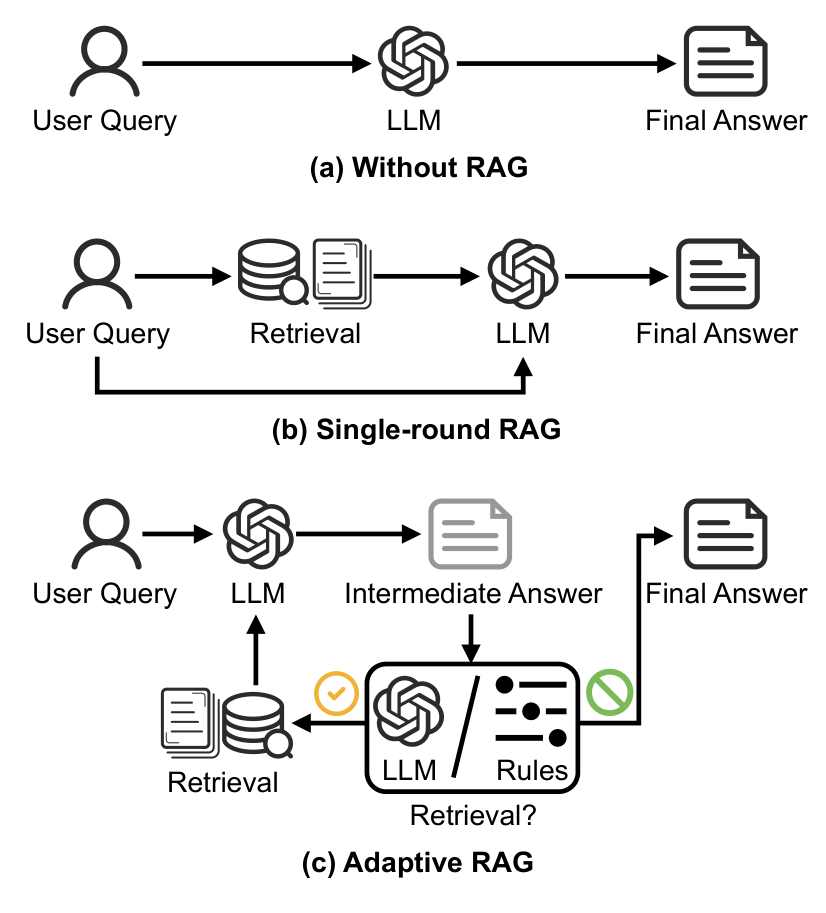
\includegraphics[height=0.78\textheight]{figures/fig7_pipelines.png}\\[2pt]
        \figcap{Figure 7. Overall pipelines for different RAG frameworks.}
      \end{center}
    \end{column}
  \end{columns}
\end{frame}

% ---------------------------------------------------------------------
% FLARE (adaptive RAG baseline 1)
% ---------------------------------------------------------------------
\begin{frame}{FLARE: forward-looking, confidence-triggered retrieval}
  \framesubtitle{Draft the upcoming sentence; retrieve only where it is uncertain \;[Jiang et al., EMNLP 2023]}
  \vfill
  \begin{center}
  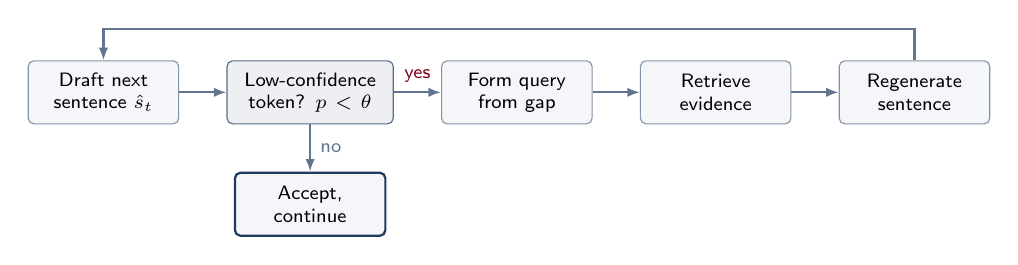
\begin{tikzpicture}[
    font=\scriptsize,
    box/.style={draw=accent!55, fill=boxbg, rounded corners=2pt, inner sep=3pt, align=center, minimum height=8mm, text width=17mm},
    dec/.style={draw=accent!75, fill=accent!8, rounded corners=2pt, inner sep=3pt, align=center, minimum height=8mm, text width=19mm},
    good/.style={box, draw=accent, line width=0.8pt},
    ar/.style={-{Latex[length=1.6mm]}, accent!70, thick}
  ]
    \node[box] (n1) {Draft next sentence $\hat{s}_t$};
    \node[dec, right=6mm of n1] (d) {Low-confidence token? $p<\theta$};
    \node[box, right=6mm of d] (q) {Form query from gap};
    \node[box, right=6mm of q] (r) {Retrieve evidence};
    \node[box, right=6mm of r] (g) {Regenerate sentence};
    \node[good, below=6mm of d] (acc) {Accept, continue};
    \draw[ar] (n1)--(d);
    \draw[ar] (d)--node[above, text=crimson]{yes} (q);
    \draw[ar] (q)--(r);
    \draw[ar] (r)--(g);
    \draw[ar] (d)--node[right]{no} (acc);
    \draw[ar] (g.north) -- ++(0,4mm) -| (n1.north);
  \end{tikzpicture}\\[2pt]
  \figcap{Schematic of the FLARE (direct) loop — cf.\ Fig.~1, Jiang et al., 2023.}
  \end{center}
  \vfill
  \begin{columns}[T]
    \begin{column}{0.55\textwidth}
      \begin{itemize}\setlength{\itemsep}{5pt}
        \item \textbf{Forward-looking} — drafts the next sentence to \good{\emph{anticipate}} evidence needs.
        \item \textbf{Active trigger} — retrieves only when a token probability $<\theta$.
        \item \textbf{Query from the gap} — mask the low-confidence span; \emph{inference-time, no training}.
      \end{itemize}
    \end{column}
    \begin{column}{0.45\textwidth}
      \begin{tcolorbox}[title={Limitation $\rightarrow$ MA-RAG}]
        Token confidence is \warn{\emph{noisy}} — trivial tokens dominate; \warn{\emph{confident hallucinations}} never trigger retrieval.\\[3pt]
        {\color{muted}MA-RAG reads \emph{semantic conflict} among candidate answers instead.}
      \end{tcolorbox}
    \end{column}
  \end{columns}
  \vfill
\end{frame}

% ---------------------------------------------------------------------
% TC-RAG (adaptive RAG baseline 2)
% ---------------------------------------------------------------------
\begin{frame}{TC-RAG: a Turing-complete, stack-controlled retrieval loop}
  \framesubtitle{An LLM controller drives a memory stack; a state value gates retrieve-vs-stop \;[Jiang et al., 2024]}
  \vfill
  \begin{center}
  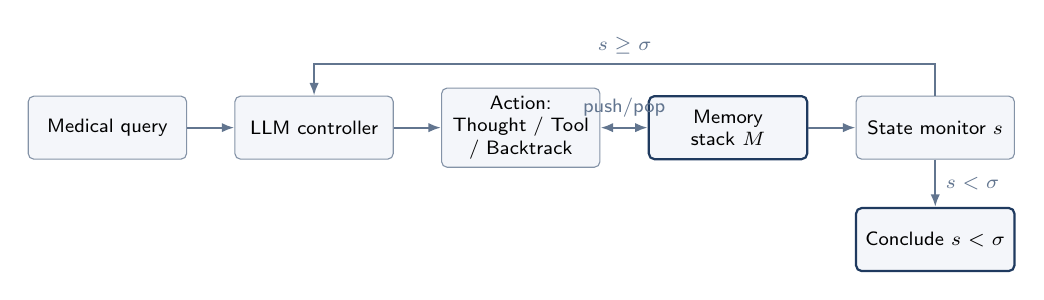
\begin{tikzpicture}[
    font=\scriptsize,
    box/.style={draw=accent!55, fill=boxbg, rounded corners=2pt, inner sep=3pt, align=center, minimum height=8mm, text width=18mm},
    good/.style={box, draw=accent, line width=0.8pt},
    ar/.style={-{Latex[length=1.6mm]}, accent!70, thick}
  ]
    \node[box] (q) {Medical query};
    \node[box, right=6mm of q] (c) {LLM controller};
    \node[box, right=6mm of c] (a) {Action: Thought / Tool / Backtrack};
    \node[good, right=6mm of a] (m) {Memory stack $M$};
    \node[box, right=6mm of m] (s) {State monitor $s$};
    \node[good, below=6mm of s] (cc) {Conclude $s<\sigma$};
    \draw[ar] (q)--(c);
    \draw[ar] (c)--(a);
    \draw[{Latex[length=1.6mm]}-{Latex[length=1.6mm]}, accent!70, thick] (a)--node[above]{push/pop} (m);
    \draw[ar] (m)--(s);
    \draw[ar] (s)--node[right]{$s<\sigma$} (cc);
    \draw[ar] (s.north) -- ++(0,4mm) -| node[near start, above]{$s\ge\sigma$} (c.north);
  \end{tikzpicture}\\[2pt]
  \figcap{Schematic of the TC-RAG controller loop — cf.\ Fig.~1, Jiang et al., 2024.}
  \end{center}
  \vfill
  \begin{columns}[T]
    \begin{column}{0.55\textwidth}
      \begin{itemize}\setlength{\itemsep}{5pt}
        \item \textbf{LLM as controller} — push/pop a \emph{memory stack} (Thought, Tool, Backtrack, Summary, Conclusion).
        \item \textbf{Turing-complete} — branching + looping + \emph{\good{state-gated}} halting.
        \item \textbf{Backtrack / Summary} — actively \emph{evict} \warn{noisy or erroneous evidence}.
      \end{itemize}
    \end{column}
    \begin{column}{0.45\textwidth}
      \begin{tcolorbox}[title={Limitation $\rightarrow$ MA-RAG}]
        Stop signal is a \emph{token-level} state (perplexity / entropy) — \warn{never checks} \emph{answer-level} correctness.\\[3pt]
        {\color{muted}MA-RAG gates on \emph{cross-candidate disagreement}, not one trajectory's tokens.}
      \end{tcolorbox}
    \end{column}
  \end{columns}
  \vfill
\end{frame}

% =====================================================================
\section{Approach: MA-RAG}
% =====================================================================

% ---------------------------------------------------------------------
% Problem definition & notation
% ---------------------------------------------------------------------
\begin{frame}{Problem definition \& notation}
  \framesubtitle{Medical QA via iterative, multi-round agentic retrieval over MedCorp}
  \vfill
  \begin{columns}[T, onlytextwidth]
    \begin{column}{0.44\textwidth}
      \begin{itemize}\setlength{\itemsep}{6pt}
        \item \textbf{Task} — medical QA (multiple-choice + open-ended), \emph{multi-step} reasoning $\to$ answer query $q$.
        \item \textbf{Retriever} — BM25 + MedCPT reranker over \emph{MedCorp} $\to$ evidence documents.
        \item \textbf{Loop} — up to $T$ rounds: sample $N$ candidates, then \good{\emph{stop when they agree}} (top consensus $\ge\epsilon$) or \emph{retrieve} \good{targeted evidence} and continue.
      \end{itemize}
    \end{column}
    \hfill
    \begin{column}{0.48\textwidth}
      \scriptsize
      \renewcommand{\arraystretch}{1.3}
      \setlength{\tabcolsep}{5pt}
      \begin{tabular}{@{}r @{\ \ } >{\raggedright\arraybackslash}p{0.84\textwidth}@{}}
        \toprule
        \multicolumn{2}{@{}l}{\textbf{Notation}}\\
        \midrule
        $q$ & medical query\\
        $M$ & LLM backbone (shared by agents)\\
        $I$ & fixed task instruction\\
        $D_t$ & retrieved documents at round $t$ (evolving)\\
        $H_t$ & ranked history, $\mathrm{Rank}(A_{t-1})$\\
        $A_t$ & $N$ candidate answers $\{a_t^1,\dots,a_t^N\}$\\
        $N$ & candidates per round\\
        $T$ & max refinement rounds (def.\ 8)\\
        $K$ & retrieval queries per round (def.\ 4)\\
        $\epsilon$ & consensus threshold (gates retrieval)\\
        \bottomrule
      \end{tabular}
    \end{column}
  \end{columns}
  \vfill
\end{frame}

% ---------------------------------------------------------------------
% Key idea (제안하는 방법 — 핵심 아이디어)
% ---------------------------------------------------------------------
\begin{frame}{Key idea: disagreement reveals the knowledge gap}
  \framesubtitle{Semantic conflict among candidate answers is a grounded retrieval signal}
  \vfill
  \begin{center}
  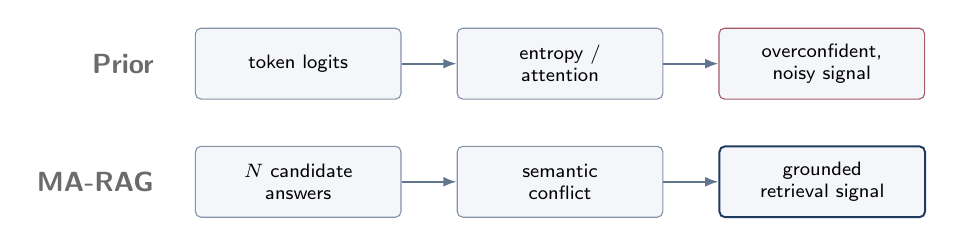
\begin{tikzpicture}[
    font=\scriptsize,
    box/.style={draw=accent!55, fill=boxbg, rounded corners=2pt, inner sep=3pt,
                align=center, minimum height=9mm, text width=24mm},
    bad/.style={box, draw=crimson!65},
    good/.style={box, draw=accent, line width=0.7pt},
    lane/.style={font=\bfseries, text=muted, anchor=east},
    ar/.style={-{Latex[length=1.7mm]}, accent!70, thick}
  ]
    \node[lane] (pl) at (0,1.5) {Prior};
    \node[box, right=4mm of pl] (p1) {token logits};
    \node[box, right=7mm of p1] (p2) {entropy /\\ attention};
    \node[bad, right=7mm of p2] (p3) {overconfident,\\ noisy signal};
    \draw[ar] (p1)--(p2);  \draw[ar] (p2)--(p3);
    \node[lane] (ml) at (0,0) {MA-RAG};
    \node[box, right=4mm of ml] (m1) {$N$ candidate\\ answers};
    \node[box, right=7mm of m1] (m2) {semantic\\ conflict};
    \node[good, right=7mm of m2] (m3) {grounded\\ retrieval signal};
    \draw[ar] (m1)--(m2);  \draw[ar] (m2)--(m3);
  \end{tikzpicture}
  \end{center}
  \vfill
  \begin{center}Candidates \emph{conflict} $\Rightarrow$ model \warn{lacks evidence} — exactly where retrieval helps most.\end{center}
  \vfill
  \begin{tcolorbox}[title={MA-RAG in one line}]
    Conflict $\to$ \good{targeted queries} \emph{and} ranked history $\to$ iterate to \good{stable consensus} — mirroring how clinicians seek evidence when diagnoses disagree.
  \end{tcolorbox}
  \vfill
\end{frame}

% ---------------------------------------------------------------------
% Concept / running example  (Figure 1)
% ---------------------------------------------------------------------
\begin{frame}{The idea in one picture: conflict $\rightarrow$ consensus}
  \framesubtitle{A running clinical example — origin of the recurrent laryngeal nerve}
  \begin{columns}[t]
    \begin{column}{0.6\textwidth}
      \begin{center}
        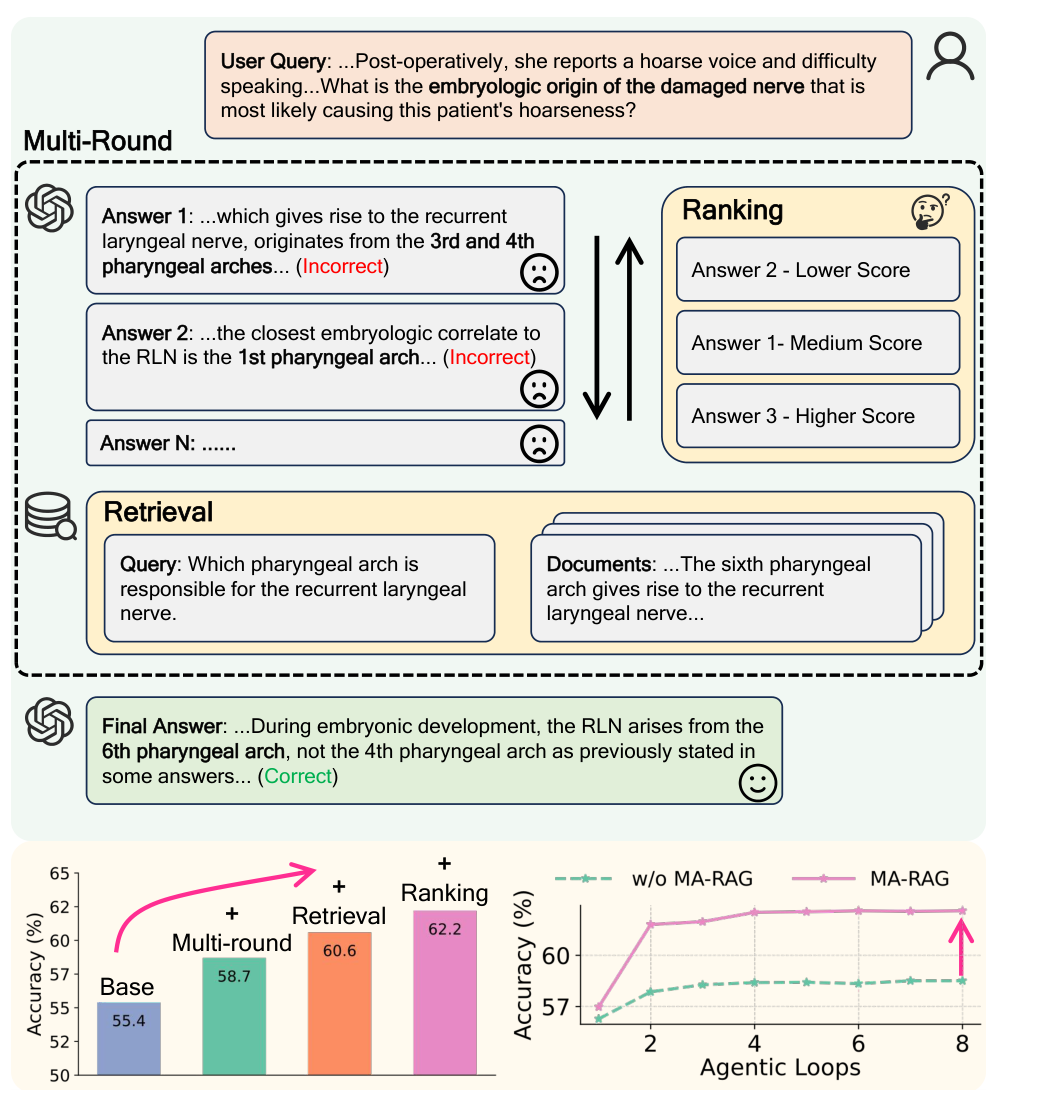
\includegraphics[height=0.58\textheight]{figures/concept.png}\\[2pt]
        \figcap{Figure 1. MA-RAG iteratively refines conflict into a unified consensus.}
      \end{center}
    \end{column}
    \begin{column}{0.4\textwidth}
      \vfill
      \textbf{Query} — embryologic origin of the nerve causing post-operative hoarseness?
      \smallskip
      \begin{itemize}\setlength{\itemsep}{7pt}
        \item Candidates \warn{\emph{disagree}}: ``3rd/4th arch'' vs.\ ``1st arch'' — \warn{both wrong}.
        \item Conflict $\Rightarrow$ query: \emph{which pharyngeal arch forms the recurrent laryngeal nerve?}
        \item Retrieve: ``the \textbf{6th} pharyngeal arch gives rise to it.''
        \item \good{Consensus}: \textbf{6th arch} — {\blue correct}.
      \end{itemize}
      \vfill
    \end{column}
  \end{columns}
  \vfill
  {\kr\scriptsize\color{muted}\textbf{한글 풀이.} 후보 답이 서로 엇갈림(1·3·4번 인두궁 — 모두 오답)은 모델이 모른다는 신호. 충돌 지점을 검색어로 만들어 근거(되돌이후두신경 = 6번 인두궁)를 찾고, 다시 풀면 6번 궁(정답)으로 수렴. \quad(arch = 인두궁: 발생기 목 구조, 번호는 머리→목 순)}
\end{frame}

% ---------------------------------------------------------------------
% Method overview  (Figure 2)
% ---------------------------------------------------------------------
\begin{frame}{MA-RAG: one agentic refinement loop}
  \framesubtitle{Three agents evolve the evidence $D_t$ and reasoning history $H_t$ each round}
  \vfill
  \begin{center}
    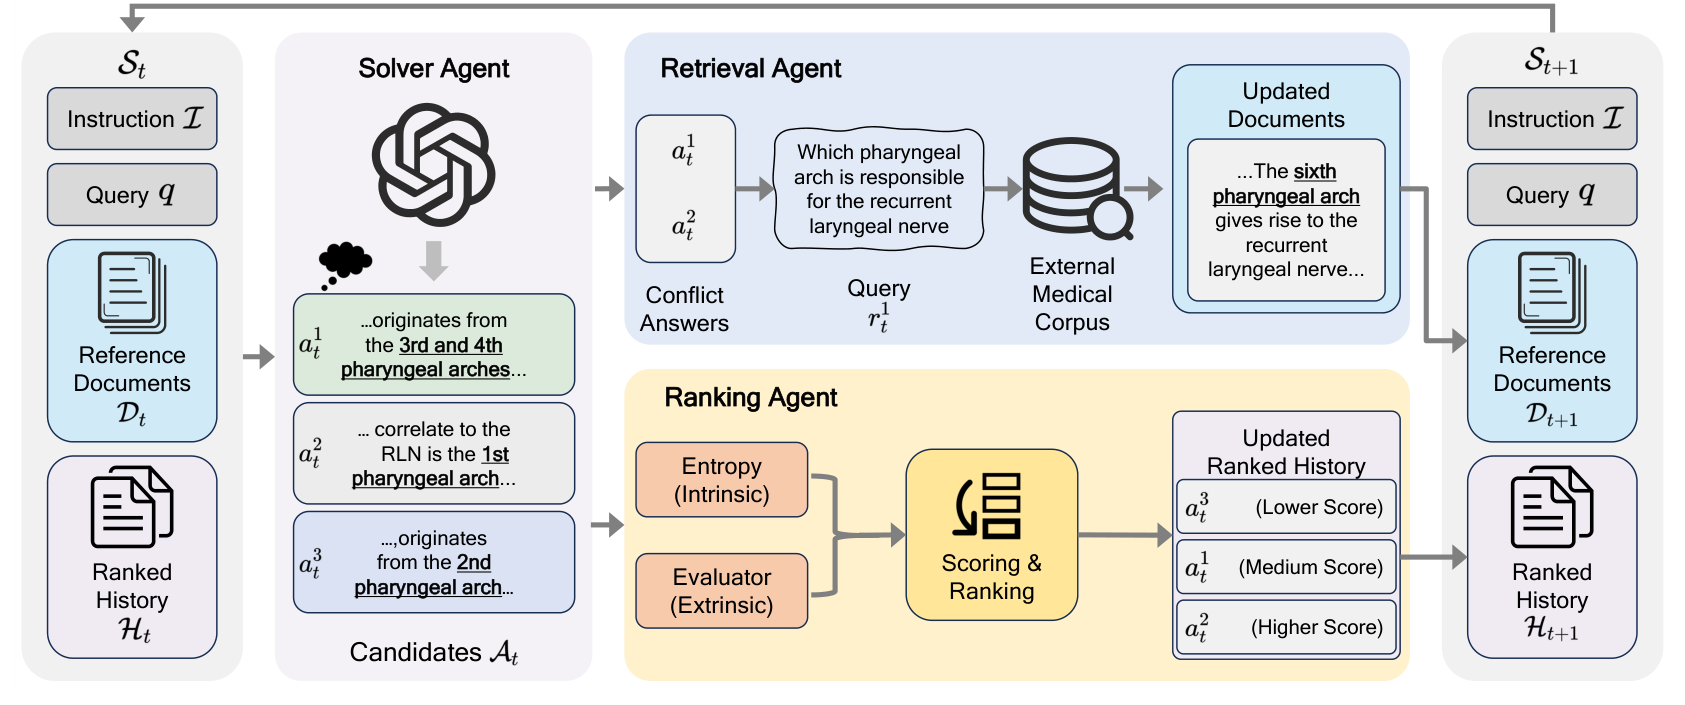
\includegraphics[width=0.88\linewidth]{figures/pipeline.png}\\[4pt]
    \figcap{Figure 2. Per round $t$: Solver $\rightarrow$ Retrieval $\rightarrow$ Ranking, evolving the state $S_t=\{I,q,D_t,H_t\}$ (notation as before).}
  \end{center}
  \vfill
  \begin{center}\small
    \warn{Conflict among candidates} $A_t$ \good{drives} \emph{both} $D_{t+1}$ (\emph{what} to retrieve) \emph{and} $H_{t+1}$ (\emph{how} to present history).
  \end{center}
  \vfill
\end{frame}

% ---------------------------------------------------------------------
% Algorithm pseudocode (Appendix Algorithm 1)
% ---------------------------------------------------------------------
\begin{frame}{Putting it together: the MA-RAG algorithm}
  \framesubtitle{Appendix Alg.\ 1 — Solver \textperiodcentered{} Retrieval \textperiodcentered{} Ranking, repeated until consensus}
  \begin{columns}[c]
    \begin{column}{0.63\textwidth}
      \begin{center}
        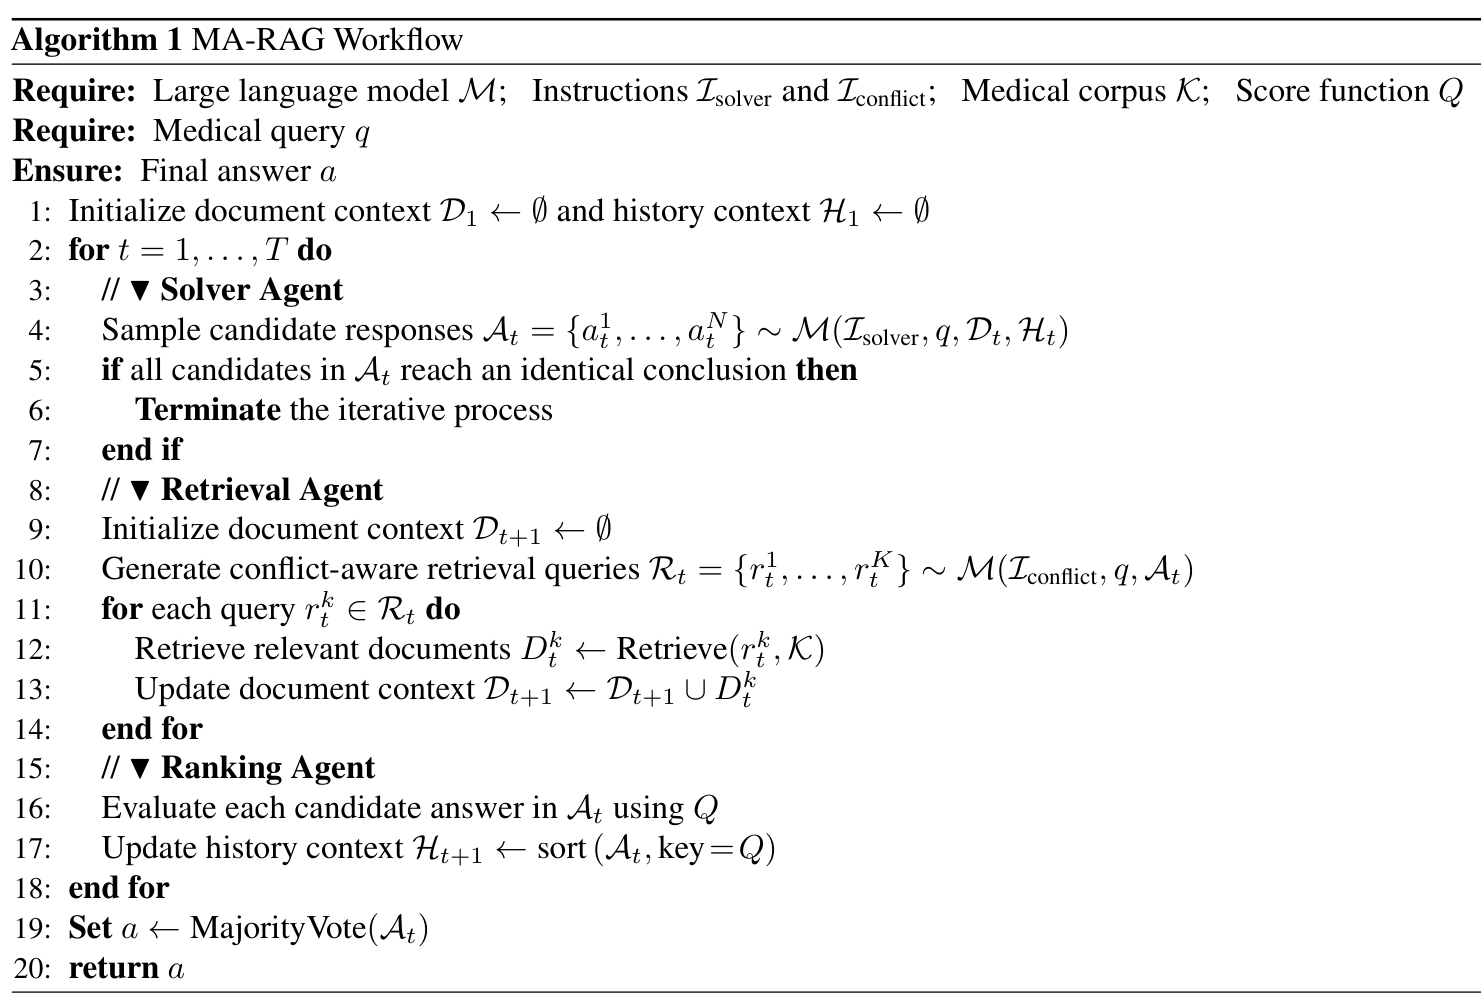
\includegraphics[width=\linewidth]{figures/algo1.png}
      \end{center}
    \end{column}
    \begin{column}{0.35\textwidth}
      \begin{itemize}\setlength{\itemsep}{9pt}
        \item Each round $t$: \good{Solver} samples $N$ candidates.
        \item \textbf{Stop early} once the candidates agree.
        \item Else \good{Retrieval} turns the conflict into $K$ queries $\to$ new evidence $D_{t+1}$.
        \item \good{Ranking} re-scores the history $H_{t+1}$ for the next round.
        \item Final answer $=$ \texttt{MajorityVote} over candidates.
      \end{itemize}
    \end{column}
  \end{columns}
\end{frame}

% ---------------------------------------------------------------------
% Solver Agent
% ---------------------------------------------------------------------
\begin{frame}{Solver: diverse candidates expose uncertainty}
  \framesubtitle{Correct chains converge; hallucinations diverge}
  \vfill
  \begin{itemize}\setlength{\itemsep}{13pt}
    \item Sample $N$ diverse candidates — temperature sampling on state $S_t$.
    \item Correct chains \good{\emph{converge}} to consensus; hallucinations \warn{\emph{diverge}}.
    \item \textbf{Stop} when consensus $\ge \epsilon$ — aggregate as final answer.
  \end{itemize}
  \vfill
  \begin{tcolorbox}[title={Candidate generation \;(Eq.~2)}]
    \[ A_t = \{a_t^1, a_t^2, \dots, a_t^N\} \sim M(I_{\text{solver}},\, q,\, D_t,\, H_t) \]
  \end{tcolorbox}
  \vfill
\end{frame}

% ---------------------------------------------------------------------
% Retrieval Agent
% ---------------------------------------------------------------------
\begin{frame}{Retrieval: conflict becomes targeted queries}
  \framesubtitle{A grounded gap signal, not token noise}
  \vfill
  \begin{itemize}\setlength{\itemsep}{13pt}
    \item Conflict pinpoints the \warn{\emph{knowledge gap}} — consistency $\Rightarrow$ enough knowledge; conflict $\Rightarrow$ \warn{missing evidence}.
    \item Extract conflicts $I_{\text{conflict}}$ $\to$ $K$ targeted queries $\to$ new evidence $D_{t+1}$ (BM25).
    \item \good{Progressively narrows} the gap each round.
  \end{itemize}
  \vfill
  \begin{tcolorbox}[title={Conflict-guided retrieval \;(Eq.~3)}]
    \[ R_t = \{r_t^1, \dots, r_t^K\} \sim M(I_{\text{conflict}},\, q,\, A_t)\;\;\Rightarrow\;\; D_{t+1} \]
  \end{tcolorbox}
  \vfill
\end{frame}

% ---------------------------------------------------------------------
% Ranking Agent
% ---------------------------------------------------------------------
\begin{frame}{Ranking: reorder history vs.\ lost-in-the-middle}
  \framesubtitle{A context optimizer that prioritizes high-quality traces}
  \vfill
  \begin{itemize}\setlength{\itemsep}{13pt}
    \item Long prompts $\to$ \warn{\emph{lost-in-the-middle}}: central reasoning cues overlooked.
    \item Score \& sort $A_{t-1}$ descending $\to$ history $H_t$ as \good{prioritized in-context demos}.
    \item Two scores $Q(\cdot)$: \good{cheap} \emph{intrinsic} entropy \textperiodcentered{} learned \emph{extrinsic} verifier (next).
  \end{itemize}
  \vfill
  \begin{tcolorbox}[title={Ranked history \;(Eq.~4)}]
    \[ H_t = \mathrm{sort}\big(A_{t-1},\, \text{key}{=}Q\big),\quad Q(a^{(1)}_{t-1}) \ge \dots \ge Q(a^{(N)}_{t-1}) \]
  \end{tcolorbox}
  \vfill
\end{frame}

% ---------------------------------------------------------------------
% Ranking score functions  (Figure 4)
% ---------------------------------------------------------------------
\begin{frame}{Two score functions: entropy vs.\ a learned verifier}
  \framesubtitle{Both rank prior traces by quality; the learned verifier separates correct from incorrect more sharply}
  \begin{columns}[t]
    \begin{column}{0.54\textwidth}
      \textbf{Intrinsic} — token entropy, \emph{free} \hfill{\footnotesize\color{muted}Eq.~5}
      \[ \textstyle Q_{\text{int}}(a) = -\tfrac{1}{L}\sum_{i=1}^{L}\mathcal{H}\!\big(P(x_i\mid x_{<i},S_t)\big) \]
      {\footnotesize Confident-but-\warn{wrong} answers stay low-entropy $\Rightarrow$ slip past.}
      \medskip

      \textbf{Extrinsic} — learned verifier $V_\theta$ \hfill{\footnotesize\color{muted}Eq.~6--7}
      \[ \textstyle Q_{\text{ext}}(a) = V_\theta(q,a) \]
      {\footnotesize ModernBERT-149M, BCE-trained on query--response pairs $D_{qa}$ (Eq.~6); \good{catches confident hallucination} ($+1.2$ pts).}
    \end{column}
    \begin{column}{0.46\textwidth}
      \begin{center}
        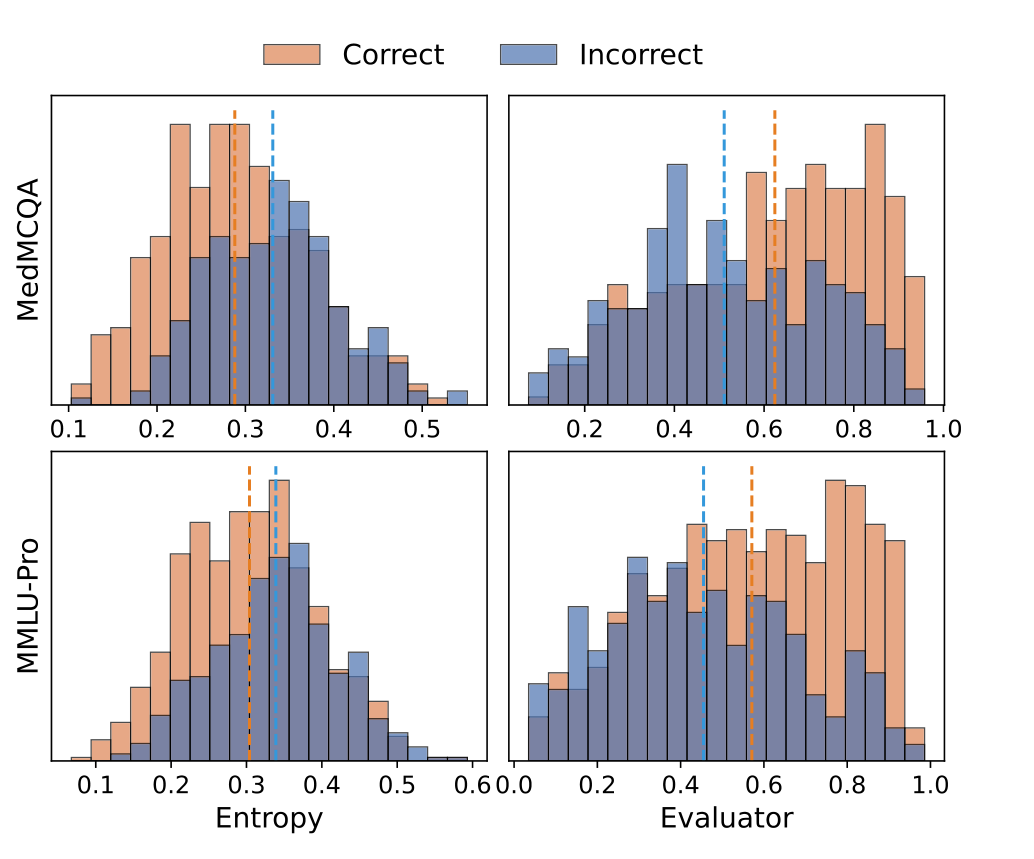
\includegraphics[width=0.86\linewidth]{figures/density.png}\\[2pt]
        \figcap{Figure 4. Score density of correct vs.\ incorrect responses (MedMCQA, MMLU-Pro).}
      \end{center}
    \end{column}
  \end{columns}
\end{frame}

% =====================================================================
\section{Experiments}
% =====================================================================

% ---------------------------------------------------------------------
% Setup
% ---------------------------------------------------------------------
\begin{frame}{Setup: 7 benchmarks, one fair retrieval stack}
  \framesubtitle{All RAG methods share an identical BM25 + MedCPT pipeline}
  \vfill
  \renewcommand{\arraystretch}{1.55}
  \setlength{\tabcolsep}{5pt}
  \begin{center}
  \begin{tabular}{@{}>{\bfseries}l p{0.70\textwidth}@{}}
    \toprule
    \normalfont\textbf{Component} & \textbf{Setup}\\
    \midrule
    Benchmarks (7) & MedQA, MedMCQA, Medbullets, MMLU-Pro, NEJM, MedExpQA, MedXpertQA — exam $\to$ \good{expert-level}\\
    Baselines (13) & 5 paradigms: 4 backbones \textperiodcentered{} 3 test-time scaling \textperiodcentered{} 3 naive RAG \textperiodcentered{} 2 adaptive RAG \textperiodcentered{} MDAgents\\
    Backbone & Qwen3-8B (best of 4), scaled to 32B\\
    Retrieval & \good{\emph{shared}}: BM25 + MedCPT reranker over MedCorp; top-128 $\to$ top-8 \;($T{=}8,\ K{=}4$)\\
    Metric & Accuracy (\%)\\
    \bottomrule
  \end{tabular}
  \end{center}
  \vfill
\end{frame}

% ---------------------------------------------------------------------
% Main results  (Table 1, full)
% ---------------------------------------------------------------------
\begin{frame}{MA-RAG-ext leads on every benchmark}
  \framesubtitle{Table 1. Accuracy (\%) on 7 medical Q\&A benchmarks}
  \begin{center}
  \scriptsize
  \renewcommand{\arraystretch}{1.05}
  \setlength{\tabcolsep}{3.2pt}
  \begin{tabular}{l ccccccc c}
    \toprule
    \textbf{Method} & MedQA & MedMCQA & Medbul. & MMLU-Pro & NEJM & MedExpQA & MedXpert & \textbf{Avg.}\\
    \midrule
    \multicolumn{9}{@{}l}{\itshape\color{muted} Backbones (8B)}\\
    Qwen3-8B            & 71.1 & 61.3 & 51.0 & 64.9 & 56.0 & 67.2 & 16.1 & 55.4\\
    Llama-3.1-8B        & 68.1 & 58.1 & 47.1 & 58.0 & 50.5 & 67.2 & 12.4 & 51.6\\
    UltraMedical-3.1-8B & 69.6 & 56.5 & 54.5 & 48.5 & 41.5 & 66.4 & 13.1 & 50.0\\
    HuatuoGPT-o1-8B     & 71.1 & 60.2 & 50.6 & 54.0 & 47.9 & 63.2 & 15.5 & 51.8\\
    \midrule
    \multicolumn{9}{@{}l}{\itshape\color{muted} Test-time scaling (Qwen3-8B)}\\
    CoT          & 69.3 & 60.3 & 50.6 & 63.4 & 56.2 & 72.0 & 18.0 & 55.7\\
    SC           & 73.3 & 62.4 & 51.9 & 66.5 & 56.6 & 70.4 & 15.7 & 56.7\\
    MDAgents     & 72.1 & 67.5 & 52.2 & 65.7 & 57.1 & 74.4 & 18.2 & 58.2\\
    Multi-Refine & 74.7 & 63.6 & 55.8 & 69.1 & 58.0 & 73.6 & 16.3 & 58.7\\
    \midrule
    \multicolumn{9}{@{}l}{\itshape\color{muted} RAG (Qwen3-8B)}\\
    SR-RAG     & 69.9 & 64.4 & 49.4 & 66.1 & 57.6 & 72.8 & 17.3 & 56.8\\
    FL-RAG     & 69.6 & 63.3 & 52.3 & 64.1 & 57.2 & 69.6 & 17.0 & 56.2\\
    FS-RAG     & 68.0 & 61.3 & 51.3 & 59.5 & 53.1 & 67.2 & 16.5 & 53.8\\
    FLARE      & 72.7 & 61.7 & 51.9 & 62.2 & 55.3 & 71.2 & 17.7 & 56.1\\
    TC-RAG     & 70.0 & 64.6 & 49.0 & 63.6 & 57.7 & 75.2 & 18.0 & 56.9\\
    MA-RAG-int & 77.0 & 67.1 & 57.1 & 70.9 & 60.8 & 72.8 & 21.2 & 61.0\\
    \rowcolor{accent!12}
    \textbf{MA-RAG-ext} & \textbf{77.1} & \textbf{67.2} & \textbf{59.1} & \textbf{70.7} & \textbf{60.5} & \textbf{78.4} & \textbf{22.2} & \textbf{62.2}\\
    \bottomrule
  \end{tabular}
  \end{center}
  \vspace{1pt}
  \begin{center}\begin{minipage}{0.95\linewidth}\centering
  \figcap{MA-RAG-ext: {\blue +6.8} vs backbone, {\blue +5.3} vs best RAG (TC-RAG), {\hl 37\%} relative on MedXpertQA.}
  \end{minipage}\end{center}
\end{frame}

% ---------------------------------------------------------------------
% Test-time scaling  (Figure 3)
% ---------------------------------------------------------------------
\begin{frame}{Test-time scaling: MA-RAG keeps improving}
  \framesubtitle{Multi-Refine plateaus; MA-RAG gains continuously across rounds}
  \vfill
  \begin{center}
    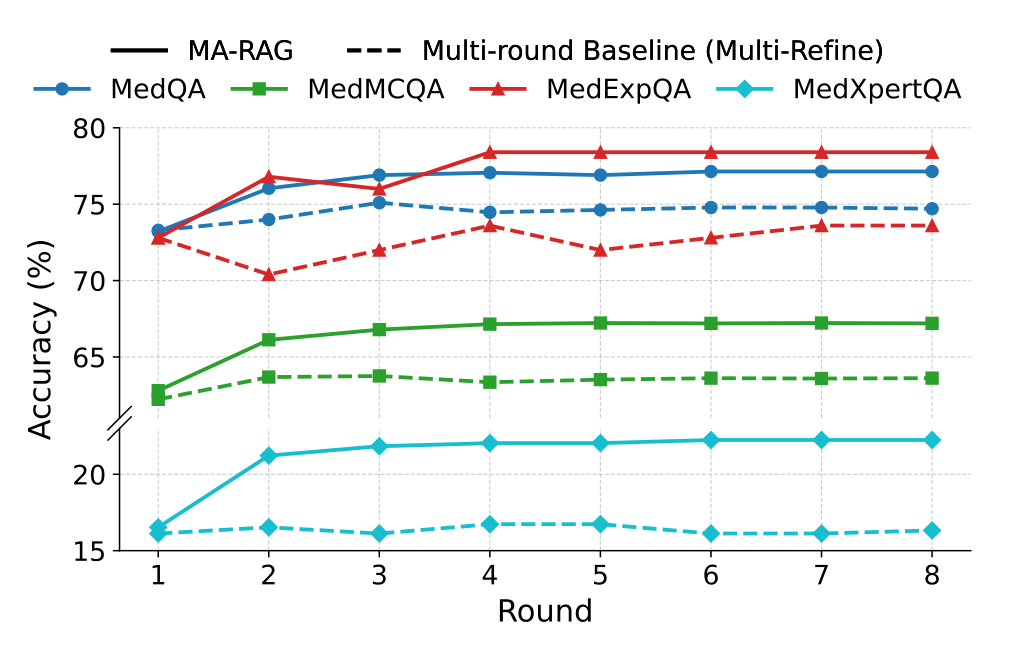
\includegraphics[width=0.62\linewidth]{figures/scaling.png}\\[4pt]
    \figcap{Figure 3. MA-RAG vs.\ the multi-round baseline (Multi-Refine) across rounds — Multi-Refine \warn{plateaus}, MA-RAG keeps \good{improving} ({\hl +37\%} on MedXpertQA).}
  \end{center}
  \vfill
\end{frame}

% ---------------------------------------------------------------------
% Ablation  (Table 2 + Table 4)
% ---------------------------------------------------------------------
\begin{frame}{Every component contributes — at 8B and 32B}
  \framesubtitle{Tables 2 \& 4. Cumulative component ablation (Avg.\ shown per benchmark)}
  \scriptsize
  \renewcommand{\arraystretch}{1.05}
  \setlength{\tabcolsep}{3.2pt}
  \begin{center}
  \textbf{\color{accent} Qwen3-8B backbone \;(Table 2)}\\[2pt]
  \begin{tabular}{l ccccccc c}
    \toprule
    \textbf{Method} & MedQA & MedMCQA & Medbul. & MMLU-Pro & NEJM & MedExpQA & MedXpert & \textbf{Avg.}\\
    \midrule
    Qwen3-8B          & 71.1 & 61.3 & 51.0 & 64.9 & 56.0 & 67.2 & 16.1 & 55.4\\
    +Multi-Refine     & 74.7 & 63.6 & 55.8 & 69.1 & 58.0 & 73.6 & 16.3 & 58.7\\
    +Retrieval Agent  & 77.1 & 66.2 & 57.5 & 69.6 & 60.3 & 74.4 & 19.2 & 60.6\\
    \rowcolor{accent!12}
    +Ranking Agent    & \textbf{77.1} & \textbf{67.2} & \textbf{59.1} & \textbf{70.7} & \textbf{60.5} & \textbf{78.4} & \textbf{22.2} & \textbf{62.2}\\
    \bottomrule
  \end{tabular}
  \\[6pt]
  \textbf{\color{accent} Qwen3-32B backbone \;(Table 4)}\\[2pt]
  \begin{tabular}{l ccccccc c}
    \toprule
    \textbf{Method} & MedQA & MedMCQA & Medbul. & MMLU-Pro & NEJM & MedExpQA & MedXpert & \textbf{Avg.}\\
    \midrule
    Qwen3-32B         & 80.8 & 68.8 & 63.0 & 73.1 & 64.4 & 82.4 & 20.2 & 64.7\\
    +Multi-Refine     & 83.6 & 70.9 & 64.9 & 75.5 & 68.4 & 86.4 & 21.2 & 67.3\\
    +Retrieval Agent  & 83.5 & 72.8 & 70.8 & 76.3 & 69.2 & 86.4 & 24.9 & 69.1\\
    \rowcolor{accent!12}
    +Ranking Agent    & \textbf{85.3} & \textbf{73.4} & \textbf{71.4} & \textbf{76.7} & \textbf{70.4} & \textbf{87.2} & \textbf{27.3} & \textbf{70.2}\\
    \bottomrule
  \end{tabular}
  \end{center}
  \vspace{1pt}
  \figcap{\;\;+Multi-Refine {\blue +3.3}, +Retrieval {\blue +1.9}, +Ranking {\blue +1.6} at 8B; \good{gains hold} (+5.5) at 32B.}
\end{frame}

% ---------------------------------------------------------------------
% Test-time scaling w.r.t. T and N  (Table 3)
% ---------------------------------------------------------------------
\begin{frame}{Scaling rounds $T$ and candidate pool $N$}
  \framesubtitle{Table 3. MA-RAG-ext accuracy (\%) vs.\ $T$ and $N$}
  \vfill
  \scriptsize
  \renewcommand{\arraystretch}{1.1}
  \setlength{\tabcolsep}{3.4pt}
  \begin{center}
  \begin{tabular}{l ccccccc c}
    \toprule
    & MedQA & MedMCQA & Medbul. & MMLU-Pro & NEJM & MedExpQA & MedXpert & \textbf{Avg.}\\
    \midrule
    \multicolumn{9}{@{}l}{\itshape\color{muted} Maximum refinement rounds $T$}\\
    $T{=}1$ & 73.2 & 62.8 & 53.2 & 67.6 & 56.2 & 72.8 & 16.5 & 57.5\\
    $T{=}2$ & 76.0 & 66.1 & 60.4 & 69.8 & 60.2 & 76.8 & 21.2 & 61.5\\
    $T{=}4$ & 77.1 & 67.2 & 59.1 & 70.8 & 60.2 & 78.4 & 22.0 & 62.1\\
    $T{=}8$ & 77.1 & 67.2 & 59.1 & 70.7 & 60.5 & 78.4 & 22.2 & 62.2\\
    \midrule
    \multicolumn{9}{@{}l}{\itshape\color{muted} Candidate pool size $N$}\\
    $N{=}2$ & 74.5 & 64.7 & 54.9 & 69.8 & 56.6 & 72.0 & 17.3 & 58.5\\
    $N{=}4$ & 76.0 & 65.7 & 58.4 & 68.2 & 58.8 & 74.4 & 18.6 & 60.0\\
    $N{=}8$ & 77.1 & 67.2 & 59.1 & 70.7 & 60.5 & 78.4 & 22.2 & 62.2\\
    \bottomrule
  \end{tabular}
  \end{center}
  \vspace{12pt}
  \small
  \begin{itemize}\setlength{\itemsep}{8pt}
    \item One extra round ($T{=}2$) $\to$ {\blue +4.0}; \good{saturates} beyond $T{=}4$ $\Rightarrow$ \good{cost-effective stop}.
    \item Larger $N$ \good{helps monotonically} — richer conflict mining + better in-context demos.
  \end{itemize}
  \vfill
\end{frame}

% ---------------------------------------------------------------------
% Scaling visualized  (Figure 5 + Figure 6)
% ---------------------------------------------------------------------
\begin{frame}{More candidates, bigger backbones — both help}
  \framesubtitle{Figures 5 \& 6. Candidate-pool scaling and backbone scaling}
  \vfill
  \begin{columns}[t]
    \begin{column}{0.5\textwidth}
      \begin{center}
        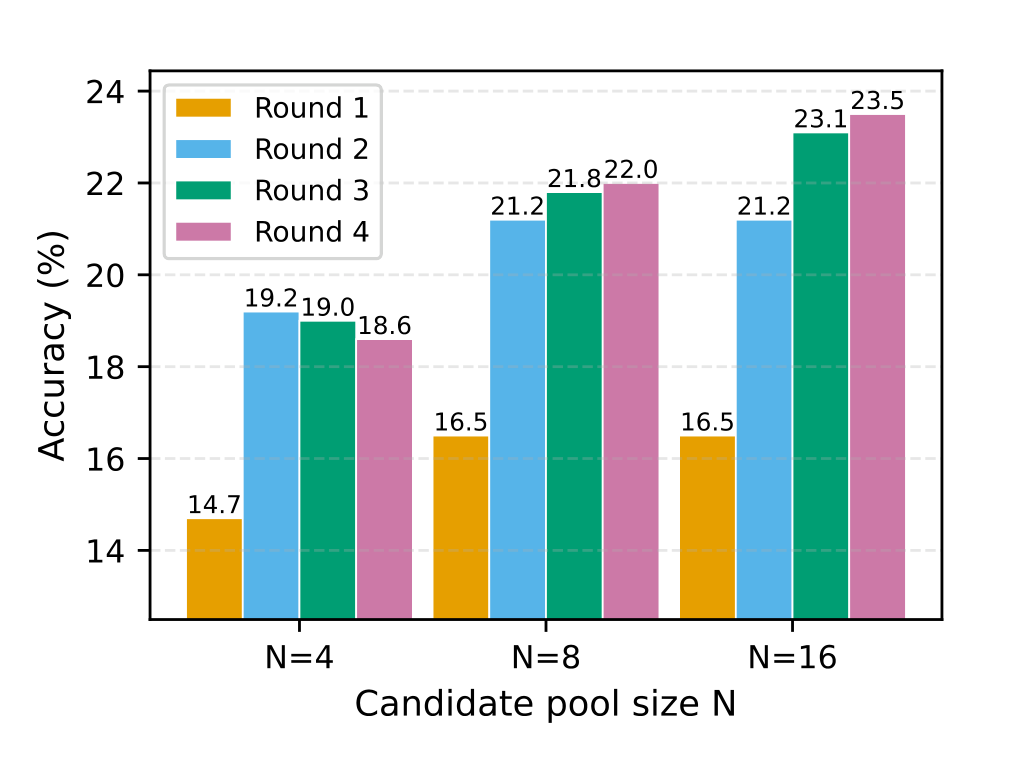
\includegraphics[width=0.86\linewidth]{figures/roundN.png}\\[3pt]
        \figcap{Figure 5. Larger $N$ \good{delays saturation} (MedXpertQA).}
      \end{center}
    \end{column}
    \begin{column}{0.5\textwidth}
      \begin{center}
        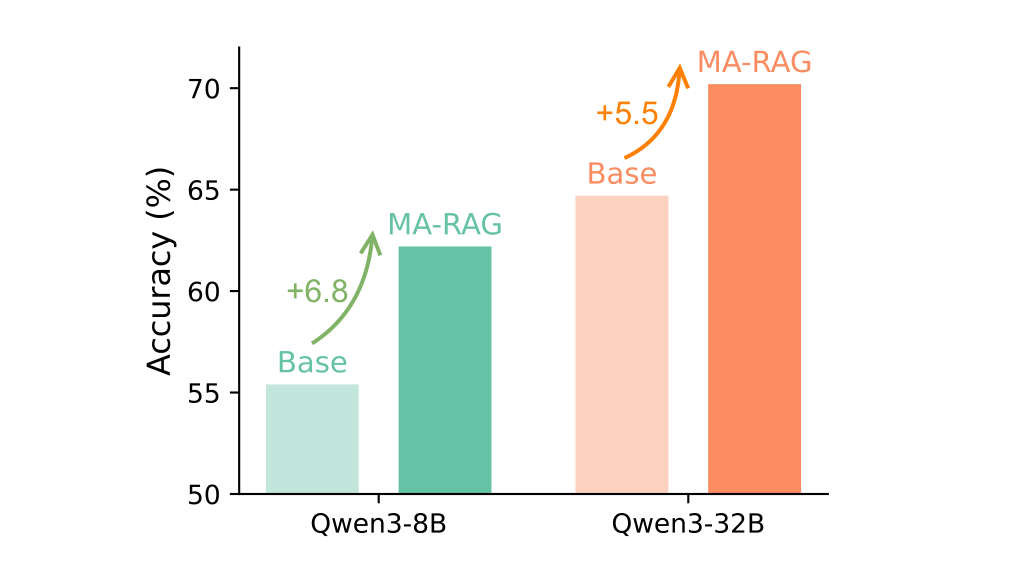
\includegraphics[width=0.86\linewidth]{figures/backbone.png}\\[3pt]
        \figcap{Figure 6. Gains across backbone scales ({\blue +6.8}/{\blue +5.5}).}
      \end{center}
    \end{column}
  \end{columns}
  \vfill
  \begin{center}
    Bigger candidate pools $\to$ improvement deeper into the loop \textperiodcentered{} \good{agentic gains persist} as the backbone scales.
  \end{center}
  \vfill
\end{frame}

% ---------------------------------------------------------------------
% Inference efficiency  (Table 5)
% ---------------------------------------------------------------------
\begin{frame}{Favorable cost--accuracy trade-off}
  \framesubtitle{Table 5. Inference efficiency on MedXpertQA (Qwen3-8B)}
  \vfill
  \begin{columns}[c]
    \begin{column}{0.56\textwidth}
      \centering
      \scriptsize
      \renewcommand{\arraystretch}{1.3}
      \setlength{\tabcolsep}{5pt}
      \begin{tabular}{l rrr r}
        \toprule
        \textbf{Method} & Docs & Gen.\ tok. & Time(s) & Acc.\\
        \midrule
        Base (Qwen3-8B) & 0    & 514    & 5.6   & 16.1\\
        SC              & 0    & 10{,}095 & 28.0  & 15.7\\
        FLARE           & 30.0 & 962    & 42.7  & 17.7\\
        TC-RAG          & 11.5 & 1{,}260  & 44.5  & 18.0\\
        MDAgents        & 8.0  & 7{,}546  & 146.2 & 18.2\\
        \rowcolor{accent!12}
        \textbf{MA-RAG-ext} & 13.7 & 12{,}762 & 70.7 & \textbf{22.2}\\
        \bottomrule
      \end{tabular}
    \end{column}
    \begin{column}{0.44\textwidth}
      \begin{itemize}\setlength{\itemsep}{16pt}
        \item \textbf{$<$ half} MDAgents' time, {\blue +4.0} accuracy.
        \item \textbf{$<$ half} FLARE's documents, {\blue +4.5} accuracy.
        \item Compute spent on \good{\emph{evidence-grounded}} refinement — not \warn{blind resampling}.
      \end{itemize}
    \end{column}
  \end{columns}
  \vfill
\end{frame}

% ---------------------------------------------------------------------
% Limitations & future work
% ---------------------------------------------------------------------
\begin{frame}{Limitations \& future work}
  \vfill
  \begin{columns}[T]
    \begin{column}{0.5\textwidth}
      {\large\bfseries\color{negmag} Limitations}
      \medskip
      \begin{itemize}\setlength{\itemsep}{14pt}
        \item \textbf{Costly inference} — $\sim$12.7k tokens, $\sim$70.7\,s / question.
        \item \textbf{Corpus-bound} — incomplete, \warn{outdated}, or institution-biased coverage.
        \item \textbf{Hallucination persists} — iteration \warn{cannot fully eliminate it}.
      \end{itemize}
    \end{column}
    \begin{column}{0.5\textwidth}
      {\large\bfseries\blue Future work}
      \medskip
      \begin{itemize}\setlength{\itemsep}{14pt}
        \item \textbf{Richer tools} — web-scale search, structured medical KBs, reasoning modules.
        \item \textbf{Sharper verifier} — ranking ceiling is tied to verifier accuracy.
        \item \textbf{Broaden \& cut cost} — beyond medicine; trim multi-round overhead.
      \end{itemize}
    \end{column}
  \end{columns}
  \vfill
\end{frame}

% =====================================================================
\section{Takeaways}
% =====================================================================

% ---------------------------------------------------------------------
% Takeaways
% ---------------------------------------------------------------------
\begin{frame}{Takeaways}
  \vfill
  \begin{itemize}\setlength{\itemsep}{20pt}
    \item {\large\bfseries\blue Conflict is signal} \;—\; semantic disagreement beats \warn{\emph{token-level uncertainty}} for steering retrieval.
    \item {\large\bfseries\blue Agentic loop scales} \;—\; evolving evidence + ranked history $\to$ {\hl +6.8 pts} over the backbone, \good{robust across rounds} \& \textbf{8B$\to$32B}.
    \item {\large\bfseries\blue Efficient grounding} \;—\; fewer docs than \textbf{FLARE}, less time than \textbf{MDAgents}, yet higher accuracy.
  \end{itemize}
  \vfill
  \begin{tcolorbox}[title={Medical-AI implication}]
    Evidence-grounded, conflict-driven refinement is a promising building block for \good{safer clinical decision support} --- best deployed as a {\bfseries human-verified assistant}.
  \end{tcolorbox}
  \vfill
\end{frame}

% ---------------------------------------------------------------------
% References
% ---------------------------------------------------------------------
\begin{frame}{References}
  \small
  \begin{thebibliography}{9}
    \bibitem{marag} Wu, W. et al.\ \emph{From Conflict to Consensus: Boosting Medical Reasoning via Multi-Round Agentic RAG}. ICML / PMLR 306, 2026.
    \bibitem{sc} Wang, X. et al.\ \emph{Self-Consistency Improves Chain-of-Thought Reasoning in Language Models}. ICLR, 2023.
    \bibitem{flare} Jiang, Z. et al.\ \emph{Active Retrieval Augmented Generation (FLARE)}. EMNLP, 2023.
    \bibitem{tcrag} Jiang, X. et al.\ \emph{TC-RAG: Turing-Complete RAG for Medical LLM Systems}. ACL, 2025.
    \bibitem{medrag} Xiong, G. et al.\ \emph{Benchmarking RAG for Medicine (MedRAG / MedCorp)}. 2024.
    \bibitem{mdagents} Kim, Y. et al.\ \emph{MDAgents: Adaptive Collaboration of LLMs for Medical Decision-Making}. NeurIPS, 2024.
  \end{thebibliography}
\end{frame}

\end{document}
